\chapter{Results}

% Eine mögliche Struktur der Arbeit sieht wie folgt aus:

% \begin{enumerate}
%     \item \textbf{Einleitung}\\
%         In der \emph{kurzen} Einleitung wird die Motivation für die Arbeit
%         dargestellt und ein Einblick in die kommenden Kapitel gegeben.
%     \item \textbf{Theoretische Grundlagen}\\
%         Alles was an theoretischen Grundlagen benötigt wird, sollte auch eher kurz gehalten werden.
%         Statt Grundlagenwissen zu präsentieren, eher auf die entsprechenden Lehrbücher verweisen.
%         Etwa: Tiefer gehende Informationen zur klassischen Mechanik entnehmen Sie bitte \cite{kuypers}.
%     \item \textbf{Ergebnisse} \\
%         Der eigentliche Teil der Arbeit, das was getan wurde.
%     \item \textbf{Zusammenfassung und Ausblick} \\
%         Zusammenfassung der Ergebnisse, Optimierungsmöglichkeiten, mögliche weitergehende Untersuchungen.
% \end{enumerate}

% Die Gliederung sollte auf der einen Seite nicht zu fein sein, auf der anderen Seite
% sollten sich klar unterscheidende Abschnitte auch kenntlich gemacht werden.

% In der hier verwendeten \KOMAScript-Klasse \texttt{scrbook} ist die oberste Gliederungsebene,
% die in der Bachelorarbeit verwendet werden sollte, das \texttt{\textbackslash chapter}.

% Ein Kapitel sollte erst dann in tiefere Gliederungsebenen unterteilt werden, wenn es auch wirklich etwas zu unterteilen gibt. 
% Es sollte keine Kapitel mit nur einem Unterkapitel (\texttt{\textbackslash section}) geben.

% In dieser Vorlage ist die Tiefe des Inhaltsverzeichnisses auf \texttt{chapter} und \texttt{section} beschränkt. 
% Möchten Sie diese Beschränkung aufheben, entfernen Sie den Befehl
% \begin{verbatim}
%             \setcounter{tocdepth}{1}
% \end{verbatim}
% aus der Präambel oder ändern Sie den Zahlenwert entsprechend. Das Inhaltsverzeichnis sollte für eine Bachelorarbeit auf eine Seite passen.

\section{Analysis of the Fixed Rate Trigger}

The functionality of the FRT is described in section~\ref{sec:daq}. In the following section, the spectrum of the data aquired by the FRT will be analyzed in 
detail. In this section, an event will mean everyting that is measured within a single trigger window. A link to the exact data used can be found 
in the appendix. The following Plots give an overview of the charge distribution of the signals collected by the FRT. Firstly, the charge distribution making up a 
single event are shown in the Histograms~\ref{fig:single_charge_hist}. As expected, the counts follow a visible poisson distribution.

\begin{figure}
    \centering
    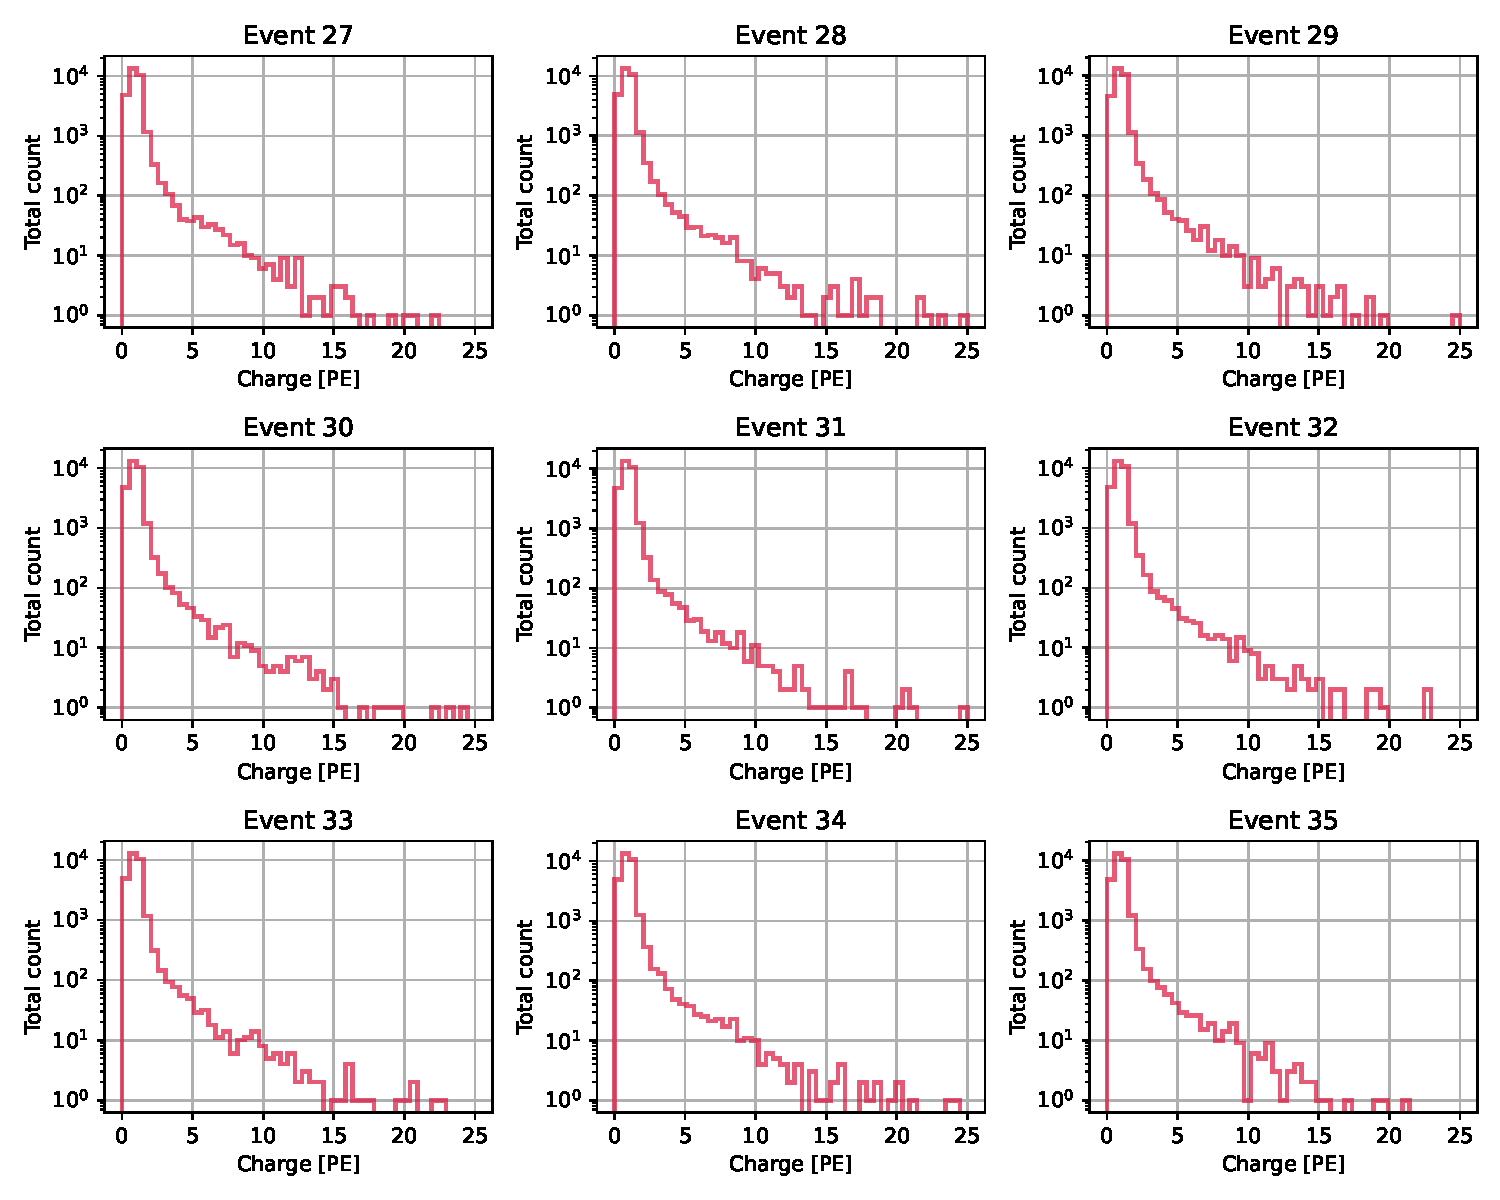
\includegraphics[width=\textwidth]{Plots/single_charge_hist.pdf}
    \caption{histograms of the charge distribution of a subset of FRT events from April 2016.}
    \label{fig:single_charge_hist}
\end{figure}
\FloatBarrier

In the histograms~\ref{fig:monthly_charge_hist} the data is grouped together in a way that shows one entry as one event where the charges are summed up, meaning the 
integrals of the histograms~\ref{fig:single_charge_hist} would each make up one event. 

\begin{figure}
    \centering
    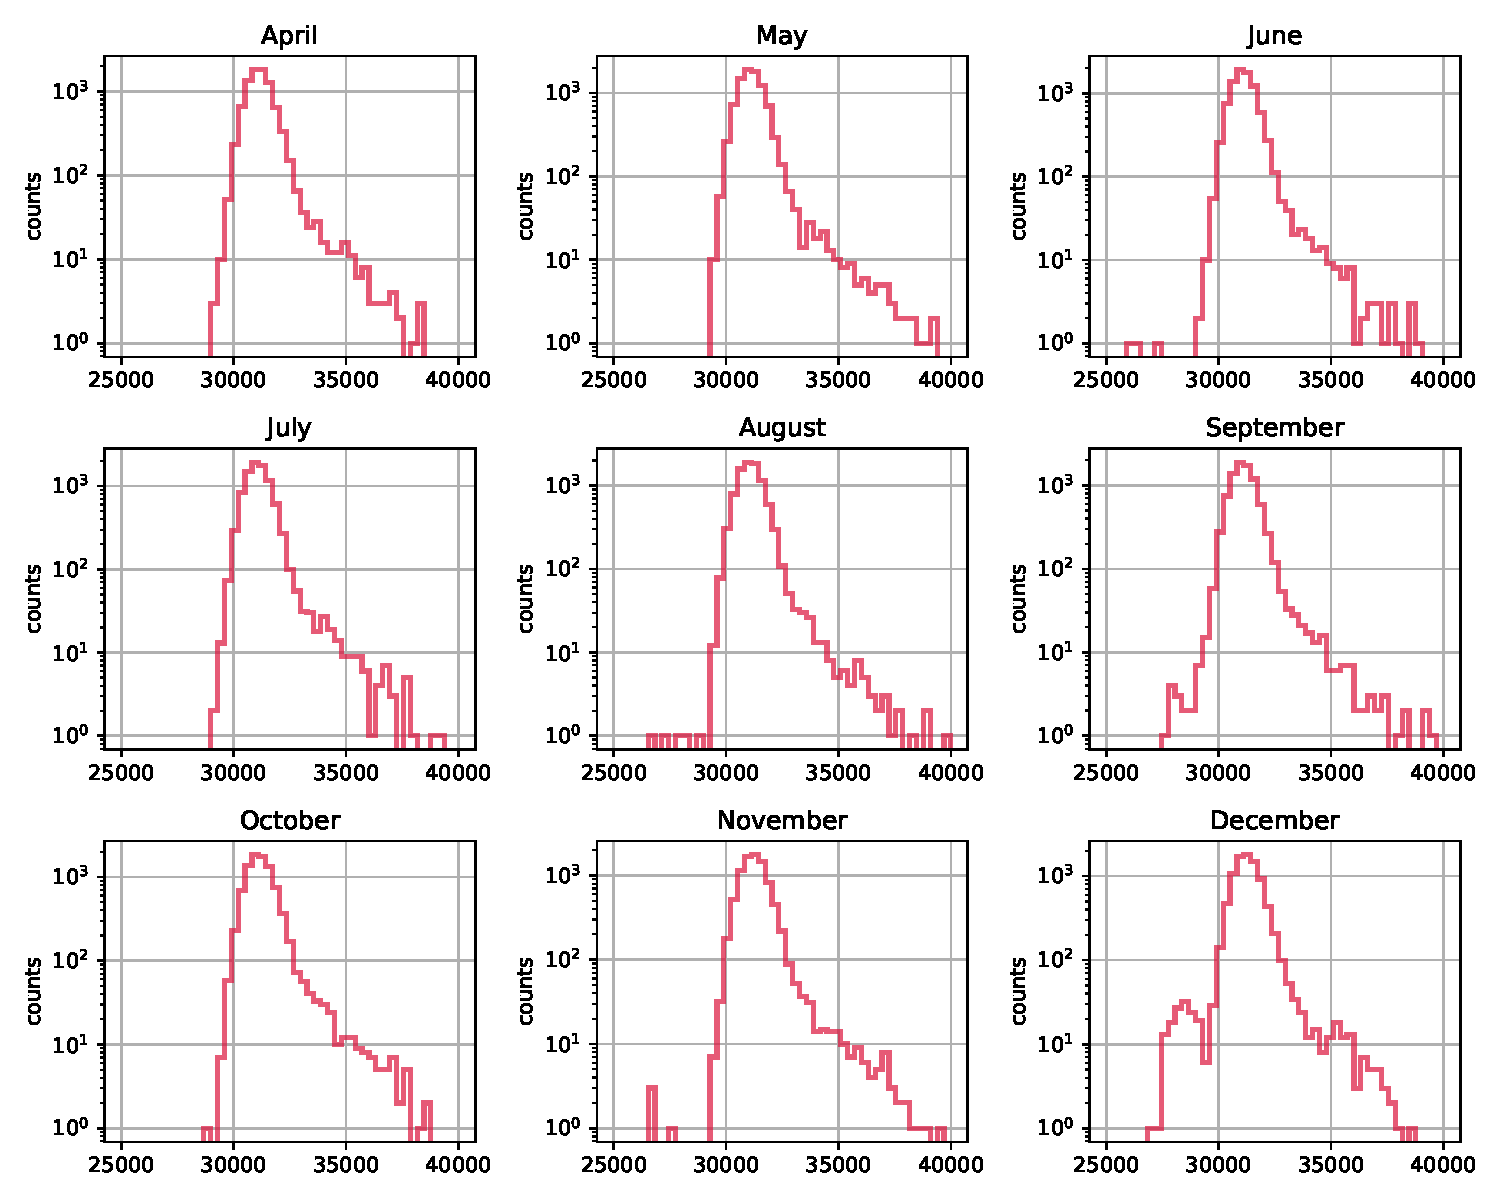
\includegraphics[width=\textwidth]{Plots/monthly_charge_hist.pdf}
    \caption{histograms of the charge distribution of all events making up entire months of 2016.}
    \label{fig:monthly_charge_hist}
\end{figure}
\FloatBarrier
Best visible in the histogram for may, up to a charge value of around \SI{3300}{PE} the count rate follows a pretty clear gaussian distribution, which is followed 
by an exponential decline. If the background noise, whatever it might be, follows a gaussian distribution, a sensible idea would be to fit a gauss for the charge 
values up to the critical point, after which the distribution type changes. Then a filter which is looking for 'real' events might filter out anything that lies 
within the fitted realm. 

\section{Muon Rate}

As explained in \ref{sec:coin} the probability function of coincidence events against total events can be estimated to follow a poisson distribution.
A theoretical distribution for different trigger windows is shown in figure(). In order to put this into a meaningful context, data() is analyzed to extract a 
connection between the event rate and other significant variable, such as energy. For muons,  